\documentclass[11pt]{article}
\usepackage[margin=1in]{geometry}
\usepackage{amsmath,amssymb}
\usepackage{graphicx}
\usepackage{booktabs}
\usepackage{xcolor}
\usepackage{tikz}
\usetikzlibrary{arrows.meta,positioning,fit,backgrounds}
\usepackage{circuitikz}
\ctikzset{transistors/scale=0.6}
\usepackage[colorlinks=true,linkcolor=blue,citecolor=blue,urlcolor=blue]{hyperref}
\usepackage{caption}
\captionsetup{font=small,labelfont=bf}

\title{\textbf{Fully In-SPICE Analog Predictive-Coding Learning for\\ Nonlinear 2D Classification: A Position Paper}}
\author{Research log, \texttt{spicenn2}}
\date{June 9, 2026}

\newcommand{\ah}{a_h}
\newcommand{\ahj}{a_{h,j}}

\begin{document}
\maketitle

\begin{abstract}
We attempt to train an analog circuit to classify three hard 2D datasets ---
\emph{circles}, \emph{rings}, \emph{spirals} --- to $>0.95$ test accuracy on each,
under a strict rule: \textbf{both inference and training run entirely inside SPICE}
(weights are charge on capacitors; the weight update is performed by transistor
multipliers; no behavioral elements), and the controller may only cycle the data.
This paper reports an honest account of what works and what does not. The two most
consequential findings are \emph{methodological}. First, the simulator dominated the
result: on the \emph{identical} netlist, ngspice reported $0.71$ on circles while
Cadence Spectre reported $0.95$ --- ngspice was materially mis-integrating the slow
capacitor-charging (learning) dynamics. Second, our own earlier numbers were inflated
$\sim0.1$ by a too-small test set and best-of-many-blocks reporting. The circuit's
learning \emph{mechanism is sound} (it trains a linearly separable control task to
$1.000$ on every random seed), and the dominant early defect (weight railing from a
common-mode mismatch) was found and fixed. The remaining, real obstacle is
\textbf{robust convergence on hard nonlinear tasks}: the features are perfectly
separable for every seed (ridge $=1.000$), yet the local delta-style rule reaches that
solution only for favorable random-feature geometries. We argue this is a delta-rule
fixed-point problem and that equilibrium propagation is the principled fix. \textbf{The
$>0.95$-on-all-three goal is not yet met.}
\end{abstract}

\section{Problem and constraints}
The goal is $>0.95$ test accuracy on \textbf{circles} (concentric annuli), \textbf{rings},
and \textbf{spirals}, subject to:
\begin{itemize}\setlength\itemsep{1pt}
\item \textbf{Inference and training are entirely in SPICE.} Weights are physical state
(differential charge on capacitor pairs). The update $\dot W \propto \varepsilon\cdot \ah$
is performed by analog cells. \emph{No behavioral elements} --- no B-source computing a
gradient, no numeric update in the controller.
\item \textbf{The controller only cycles data}: it writes the piecewise-linear schedule
that presents \texttt{(input,label)} pairs over time and supplies bias/clock voltages.
It never computes a gradient or a weight value.
\end{itemize}
This is a continuous-time predictive-coding (PC) learner realized physically.

\section{Architecture}
\label{sec:arch}
Figure~\ref{fig:arch} shows the signal flow. The hidden layer is a \emph{fixed random}
analog feature map; only the readout is trained.
\begin{figure}[h]
\centering
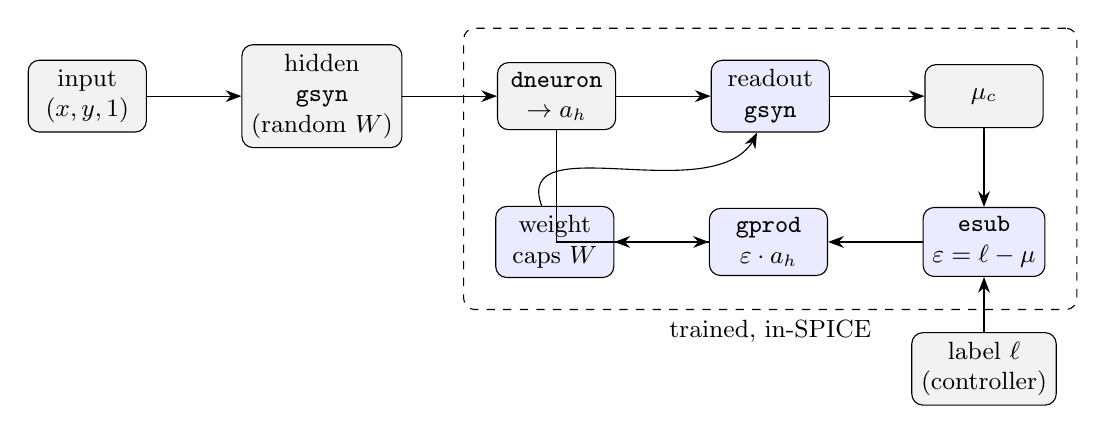
\begin{tikzpicture}[
  node distance=8mm and 12mm,
  box/.style={draw,rounded corners,minimum height=8mm,minimum width=15mm,align=center,font=\small},
  trn/.style={box,fill=blue!8},
  fix/.style={box,fill=black!5},
  >={Stealth[length=2mm]}]
\node[fix] (in) {input\\$(x,y,1)$};
\node[fix,right=of in] (gh) {hidden\\\texttt{gsyn}\\(random $W$)};
\node[fix,right=of gh] (dn) {\texttt{dneuron}\\$\to \ah$};
\node[trn,right=of dn] (gr) {readout\\\texttt{gsyn}};
\node[box,fill=black!5,right=of gr] (mu) {$\mu_c$};
\node[trn,below=10mm of mu] (es) {\texttt{esub}\\$\varepsilon=\ell-\mu$};
\node[trn,left=of es] (gp) {\texttt{gprod}\\$\varepsilon\cdot \ah$};
\node[trn,left=of gp] (cap) {weight\\caps $W$};
\node[fix,below=7mm of es] (lab) {label $\ell$\\(controller)};
\draw[->] (in)--(gh); \draw[->] (gh)--(dn); \draw[->] (dn)--(gr);
\draw[->] (gr)--(mu); \draw[->] (mu)--(es); \draw[->] (lab)--(es);
\draw[->] (es)--(gp); \draw[->] (dn) |- (gp);
\draw[->] (gp)--(cap); \draw[->] (cap) to[out=110,in=250] (gr);
\begin{scope}[on background layer]
\node[draw,dashed,rounded corners,fit=(gr)(mu)(es)(gp)(cap),inner sep=4mm,label=below:{\small trained, in-SPICE}] {};
\end{scope}
\end{tikzpicture}
\caption{Fully in-SPICE PC learner. Fixed random hidden features ($\ah$) drive a trained
readout whose weights are capacitor charge. \texttt{esub} forms the error
$\varepsilon=\ell-\mu$; \texttt{gprod} (a four-quadrant Gilbert multiplier) charges the
weight caps by the local product $\varepsilon\cdot\ah$. One \texttt{.tran} performs a
clamped training phase then a frozen evaluation phase. All cells are
transistor/R/C/V only.}
\label{fig:arch}
\end{figure}

\noindent\textbf{Cells (all pure transistor/R/C/V, LEVEL-1 MOSFETs).}
\texttt{gsyn}: source-degenerated Gilbert multiplier (synapse). \texttt{dneuron}:
differential-pair neuron with common-mode load. \texttt{esub}: two-tail differential
subtractor forming $\varepsilon_c=\ell_c-\mu_c$. \texttt{gprod}: four-quadrant Gilbert
product sourcing/sinking current into the weight caps $\propto \varepsilon_c\,\ahj$.
Signed weights are the differential charge $w=q^+-q^-$; an in-circuit hinge gate
(a soft comparator) can freeze a class's update once it is confidently correct.
Transistor-level schematics of the three core cells (\texttt{gsyn}, \texttt{esub},
\texttt{gprod}) are given in Appendix~\ref{app:cells}.

\section{Two methodological findings}

\subsection{The simulator was the bottleneck}
Running the \emph{identical} netlist and configuration through two SPICE engines gives
sharply different answers (Fig.~\ref{fig:sim}). ngspice (LEVEL-1, \texttt{method=gear},
\texttt{reltol}=2e-3) reports circles $=0.713$; Cadence Spectre (default trapezoidal,
moderate \texttt{errpreset}) reports $0.950$ on the same deck, in $\sim$5$\times$ less
wall-clock time. The Spectre result is not an output-sampling artifact (strobed output
$0.950$ vs.\ full output $0.956$). We conclude that a substantial part of what we had
been calling an ``in-circuit learning ceiling'' was an \textbf{ngspice numerical
artifact} in integrating the slow capacitor-charging dynamics. \emph{Every prior
ngspice-based negative conclusion must be re-checked on Spectre before being trusted.}

\begin{figure}[h]\centering
\includegraphics[width=\textwidth]{figs/fig_sim.pdf}
\caption{Same netlist, same configuration: ngspice vs.\ Spectre. The accuracy gap
($0.713\!\to\!0.950$) is a simulator effect, and Spectre is also faster (and completes
$H{=}160$ in 5.5\,min where ngspice times out).}
\label{fig:sim}\end{figure}

\subsection{Our own numbers were inflated}
For much of the project ``circles $\approx 0.83$'' was reported. With a proper test set
(NTE $\geq 80$) and final-accuracy reporting, the true number was $\sim0.5$--$0.73$. The
inflation came from (a) a 24-example test set (granularity $0.04$, high variance) and
(b) reporting the \emph{best} over many interval-eval blocks. \textbf{Methodology rule:}
NTE $\geq 80$, report final accuracy (not best-of-blocks), average over $\geq 3$ seeds.

\section{Results}
\begin{table}[h]\centering\small
\begin{tabular}{llll}
\toprule
Task & Setup & Result & Notes\\
\midrule
blobs (linear control) & Spectre, $H{=}48$, all seeds & \textbf{1.00 / 1.00 / 1.00} & mechanism is sound\\
circles & Spectre, $H{=}48$, seed 0 & \textbf{0.950--0.956} & meets target (one seed)\\
circles & Spectre, $H{=}48$, seeds 1,2,3 & 0.59 / 0.54 / 0.61 & \emph{not robust}\\
circles & ngspice, $H{=}48$, seed 0 & 0.713 & same deck --- simulator artifact\\
circles (capacity) & ridge on $\ah$, any seed & 1.000 & features always separable\\
rings, spirals & --- & untested & not yet attempted\\
\bottomrule
\end{tabular}
\caption{Headline results. The goal ($>0.95$ robustly on all three) is \emph{not} met.}
\end{table}

The central tension is shown in Fig.~\ref{fig:robust}: the mechanism trains a separable
task to $1.0$ on every seed, and the circles features are \emph{always} linearly
separable (ridge $=1.000$), yet the in-circuit learner reaches that solution only on
favorable random-feature seeds. This is therefore a \textbf{learning-convergence
failure}, not a feature or capacity failure. Moreover, no learning-rule knob rescues a
bad seed (Fig.~\ref{fig:levers}): gate on/off, target margin, and learning-current scale
all leave seed~1 at $0.59$--$0.60$.

\begin{figure}[h]\centering
\includegraphics[width=\textwidth]{figs/fig_robust.pdf}
\caption{Mechanism sound, robustness not. blobs trains to $1.0$ every seed; circles is
seed-fragile despite ridge $=1.0$ everywhere.}
\label{fig:robust}\end{figure}

\begin{figure}[h]\centering
\includegraphics[width=0.92\textwidth]{figs/fig_levers.pdf}
\caption{On a bad-geometry seed, none of the local learning-rule knobs move the result
off $\sim0.59$. This points at the \emph{fixed point} of the rule, not its
hyperparameters.}
\label{fig:levers}\end{figure}

\section{What works / what does not}
\textbf{Works (simulator-independent):} source-degenerated Gilbert cells; the
common-mode fix --- the dominant early defect was an \texttt{esub} common-mode mismatch
(readout $\mu$-CM $0.666$ vs.\ clamp $0.5$) that railed the weights; a separate-tail
\texttt{esub} plus a CM-pinned readout load collapsed railing $92\%\!\to\!0\%$; the
hinge gate (small real gain); and the Spectre $+$\texttt{mt} backend with
\texttt{strobeperiod} output for fast, accurate iteration. The mechanism trains the
linear control task to $1.0$ on every seed.

\noindent\textbf{Does not work (believed real, not ngspice noise):} robust convergence
on hard nonlinear tasks; learning-rule knobs do not rescue bad seeds; naive $H$-scaling
is currently broken in the harness ($H{=}120/200$ collapse to $0.500$; Spectre's
\texttt{.save} does not limit nodes, producing 100\,MB$+$ PSF files). A set of ideas
that ``failed'' on ngspice (gradient-aware/replica feature, feature compression,
attenuation, two-phase variants) are now \emph{suspect} and need clean Spectre re-runs.

\section{Related work}
The relevant literature consistently avoids ``raw SGD into a sloppy analog weight,''
favoring local rules, common-mode/reference cancellation, delayed transfer, and
freeze/threshold logic. Closest to this work:
\begin{itemize}\setlength\itemsep{1pt}
\item \textbf{Equilibrium Propagation in nonlinear resistive networks} (Kendall et al.)
--- a SPICE/Spectre analog network with \emph{local} learning where inference and
training share the same physical circuit; MNIST with 100 hidden neurons, $3.43\%$ test
error. This is the most direct template, and it speaks precisely to our open problem:
EP's update uses the same nonlinear circuit in a free and a nudged phase, so its
stationary point \emph{is} the (gradient-correct) min-error solution --- exactly what a
plain delta rule on a nonlinear readout lacks.
\item \textbf{On-chip learning in a conventional MOSFET analog NN} (arXiv:1907.00625)
--- SPICE, ordinary MOSFETs (no memristors), small benchmark; closest in component
philosophy.
\item \textbf{Mixed-precision / FeCAP--memristor training} (Nature 2018; Nature
Electronics 2025) --- separate fast inference weights from higher-precision slow
learning state; transfer every $k$ samples.
\item \textbf{IBM c-TTv2 / AGAD} (Nat.\ Commun.\ 2024) --- normalize update magnitudes;
\emph{chopper / dynamic-reference} learning to cancel offsets (the algorithmic cousin of
our common-mode fix).
\item \textbf{Silicon-synapse memristive RBM/DBN} (arXiv:2203.09046) --- binary neurons,
ternary thresholded updates, blind writes.
\end{itemize}
Two themes from this literature map directly onto our results: (i) common-mode/reference
cancellation is essential (we needed it to stop weight railing), and (ii) for nonlinear
analog readouts, a \emph{contrastive / two-phase} update (EP) is the principled way to
make the learning fixed point coincide with the min-error solution.

\section{Open problems and path forward}
\begin{enumerate}\setlength\itemsep{1pt}
\item \textbf{Robustness is the crux.} Since ridge $=1.0$ for all seeds, the target is
reachable in principle; the analog \emph{rule} must converge to it regardless of feature
geometry. The leading candidate is a true \textbf{equilibrium-propagation} update (free
$+$ nudged phase, symmetric $\pm\beta$ nudge to cancel bias), now testable accurately on
Spectre.
\item \textbf{Fix the $H$-scaling harness} (limit Spectre saved nodes; check convergence
at large $H$) so ``more features $\to$ robustness'' can be tested cleanly.
\item \textbf{Re-audit ngspice-era negatives on Spectre} --- several are likely false
negatives.
\item \textbf{rings and spirals} have not been run in-SPICE at all and must clear the
same bar.
\end{enumerate}

\section{Conclusion}
A fully in-SPICE, no-behavioral-elements predictive-coding learner was built; its update
is genuine analog charge driven by transistor multipliers, and its mechanism provably
works (1.0 on a separable control task, every seed). The dominant early defect (weight
railing from a common-mode mismatch) was diagnosed and fixed. The biggest lesson is
methodological: ngspice was materially mis-simulating the learning, and an accurate
simulator (Spectre) reaches $0.95$ on circles where ngspice reported $0.71$ --- but only
on favorable random-feature seeds. The remaining real obstacle is making the analog
learning rule converge to the (provably reachable) solution \emph{robustly}, for which
equilibrium propagation is the principled next step. \textbf{The $>0.95$-on-all-three
goal is not yet met.}

\appendix
\section{Cell schematics (transistor level)}
\label{app:cells}
All cells use LEVEL-1 NMOS/PMOS, source-degeneration resistors $R$, and a tail current
source. Differential signals are used throughout ($\cdot_p,\cdot_n$). The synapse and the
readout are the \emph{same} \texttt{gsyn} cell (Fig.~\ref{fig:gsyn}); the error neuron
\texttt{esub} (Fig.~\ref{fig:esub}) uses \emph{separate tails} per input pair so the
output depends on input \emph{differences}, not common mode --- the fix that stopped weight
railing; the learning cell \texttt{gprod} (Fig.~\ref{fig:gprod}) converts the differential
product current into capacitor charge.

\begin{figure}[h]\centering
\begin{circuitikz}[line width=0.7pt,font=\small]
\draw (-0.5,7.2) -- (9,7.2); \node[right] at (9,7.2){$V_{dd}$};
\draw (2,6.7) node[pigfete,anchor=D,xscale=-1](LP){}; \draw (LP.S)--(2,7.2);
\draw (6,6.7) node[pigfete,anchor=D](LN){}; \draw (LN.S)--(6,7.2);
\node[font=\footnotesize,align=center] at (4,7.0){\texttt{cmld}\\(CM load)};
\draw (LP.G)--(4,6.4)--(LN.G);
\draw (LP.D)--(2,6.0) node[circ](outp){}; \draw (LN.D)--(6,6.0) node[circ](outn){};
\node[left] at (1.7,6.0){$out_p$}; \node[right] at (6.3,6.0){$out_n$};
\draw (1.0,5.0) node[nigfete,anchor=D](M1){}; \draw (2.6,5.0) node[nigfete,anchor=D](M2){};
\draw (5.4,5.0) node[nigfete,anchor=D](M3){}; \draw (7.0,5.0) node[nigfete,anchor=D](M4){};
\node[font=\footnotesize,above=0pt] at (M1.D){M1}; \node[font=\footnotesize,above=0pt] at (M2.D){M2};
\node[font=\footnotesize,above=0pt] at (M3.D){M3}; \node[font=\footnotesize,above=0pt] at (M4.D){M4};
\draw (M1.D)|-(outp); \draw (M4.D)|-(6,6.0);
\draw (M2.D)|-(2.6,5.8)-|(outn); \draw (M3.D)--(5.4,6.0)--(outn);
\draw (M1.G)--++(-0.45,0) node[left]{$in_p$}; \draw (M2.G)--++(-0.45,0) node[left]{$in_n$};
\draw (M3.G)--++(-0.45,0) node[left]{$in_p$}; \draw (M4.G)--++(0.45,0) node[right]{$in_n$};
\draw (M1.S)to[R,l_=$R$]++(0,-1.1) coordinate(a1); \draw (M2.S)to[R,l=$R$]++(0,-1.1) coordinate(a2);
\draw (M3.S)to[R,l_=$R$]++(0,-1.1) coordinate(b1); \draw (M4.S)to[R,l=$R$]++(0,-1.1) coordinate(b2);
\draw (a1)--(a2); \draw (b1)--(b2);
\node[circ] at(1.8,2.8){}; \node[below=1pt] at (1.8,2.8){$n_a$};
\node[circ] at(6.2,2.8){}; \node[below=1pt] at (6.2,2.8){$n_b$};
\draw (1.8,2.2) node[nigfete,anchor=D](M5){}; \draw (6.2,2.2) node[nigfete,anchor=D](M6){};
\node[font=\footnotesize,left=0pt] at (M5.D){M5}; \node[font=\footnotesize,right=0pt] at (M6.D){M6};
\draw (M5.D)--(1.8,2.8); \draw (M6.D)--(6.2,2.8);
\draw (M5.G)--++(-0.45,0) node[left]{$w_p$}; \draw (M6.G)--++(0.45,0) node[right]{$w_n$};
\draw (M5.S)to[R,l_=$R$]++(0,-1.0) coordinate(t1); \draw (M6.S)to[R,l=$R$]++(0,-1.0) coordinate(t2);
\draw (t1)--(t2); \draw(t1)--(4,0.2)--(t2); \node[above right] at (4,0.2){$n_t$};
\draw (4,-0.5) node[nigfete,anchor=D](MT){}; \draw (MT.D)--(4,0.2);
\draw (MT.G)--++(-0.5,0) node[left]{$v_{bn}$}; \draw (MT.S)--++(0,-0.4) node[ground]{};
\node[font=\footnotesize,right=0pt] at (MT.D){M$_t$};
\end{circuitikz}
\caption{\texttt{gsyn} --- source-degenerated Gilbert multiplier. The weight pair
(M5,M6, gates $w_p,w_n$) steers the tail current; the input quad (M1--M4, gates
$in_p,in_n$) forms the product at $out_p,out_n$. Degeneration resistors $R$ linearize the
cell. Used unchanged as both the hidden synapse and the trained readout.}
\label{fig:gsyn}
\end{figure}

\begin{figure}[h]\centering
\begin{circuitikz}[line width=0.7pt,font=\small]
\draw (-0.5,5) -- (8,5) node[right]{$V_{dd}$};
\draw (1.5,5) to[R,l_=$R_L$] (1.5,4.0) node[circ](ep){}; \node[left] at (1.2,3.8){$e_p$};
\draw (6.5,5) to[R,l=$R_L$] (6.5,4.0) node[circ](en){}; \node[right] at (6.8,3.8){$e_n$};
\draw (1.0,3.2) node[nigfete,anchor=D](M1x){}; \draw (2.6,3.2) node[nigfete,anchor=D](M2x){};
\draw (M1x.D)--(1.0,4.0)-|(ep); \draw (M2x.D)--(2.6,4.0)-|(en);
\draw (M1x.G)--++(-0.4,0) node[left]{$x_n$}; \draw (M2x.G)--++(0.4,0) node[right]{$x_p$};
\draw (M1x.S)--(1.8,2.4); \draw (M2x.S)--(1.8,2.4); \node[circ] at(1.8,2.4){};
\draw (1.8,2.4)--(1.8,2.0) node[nigfete,anchor=D](MTx){};
\draw (MTx.G)--++(-0.4,0) node[left]{$v_{bn}$}; \draw (MTx.S)--++(0,-0.3) node[ground]{};
\node[font=\footnotesize] at (2.6,1.7){tail$_x$};
\draw (5.0,3.2) node[nigfete,anchor=D](M1m){}; \draw (6.6,3.2) node[nigfete,anchor=D](M2m){};
\draw (M1m.D)--(5.0,4.0)-|(ep); \draw (M2m.D)--(6.6,4.0)-|(en);
\draw (M1m.G)--++(-0.4,0) node[left]{$m_p$}; \draw (M2m.G)--++(0.4,0) node[right]{$m_n$};
\draw (M1m.S)--(5.8,2.4); \draw (M2m.S)--(5.8,2.4); \node[circ] at(5.8,2.4){};
\draw (5.8,2.4)--(5.8,2.0) node[nigfete,anchor=D](MTm){};
\draw (MTm.G)--++(-0.4,0) node[left]{$v_{bn}$}; \draw (MTm.S)--++(0,-0.3) node[ground]{};
\node[font=\footnotesize] at (6.6,1.7){tail$_m$};
\end{circuitikz}
\caption{\texttt{esub} --- separate-tail differential subtractor forming
$\varepsilon=\ell-\mu$ at $e_p-e_n$. The label clamp ($x_p,x_n$) and the readout output
($m_p,m_n$) drive two diff pairs with \emph{independent} tails into shared loads, so the
output tracks the input \emph{differences} and rejects common mode. Matching the clamp and
readout common modes here is what collapsed weight railing $92\%\!\to\!0\%$.}
\label{fig:esub}
\end{figure}

\begin{figure}[h]\centering
\begin{circuitikz}[line width=0.7pt,font=\small]
\draw (-0.5,5.4) -- (10,5.4) node[right]{$V_{dd}$};
\draw (0.0,2.5) rectangle (3.2,4.5);
\node[align=center] at (1.6,3.6){Gilbert\\product core\\\footnotesize(\texttt{gsyn} topology)};
\draw (0.0,4.1)--(-1.2,4.1) node[left]{$x_p,x_n=\varepsilon_c$};
\draw (0.0,2.9)--(-1.2,2.9) node[left]{$y_p,y_n=a_{h,j}$};
\draw (3.2,4.1)--(4.0,4.1) node[circ]{} coordinate(iop); \node[above] at (3.9,4.2){$i_{op}$};
\draw (3.2,2.9)--(4.6,2.9) coordinate(ionin); \node[above] at (3.9,3.0){$i_{on}$};
\draw (4.6,2.4) rectangle (6.2,3.4); \node[align=center,font=\footnotesize] at (5.4,2.9){$i_{on}$\\mirror};
\draw (8.0,4.5) node[pigfete,anchor=S,xscale=-1](PU){}; \draw (PU.S)--(8.0,5.4);
\node[above,font=\footnotesize] at (7.5,4.9){push};
\draw (PU.G) -- (5.0,4.5) -- (5.0,4.1) -- (iop);
\draw (PU.D)--(8.0,3.2) node[circ](wp){}; \node[right] at (8.25,3.25){$w_p$};
\draw (wp)--(9.3,3.2) to[C,l=$C_w$](9.3,1.7) node[ground]{};
\draw (8.0,2.1) node[nigfete,anchor=D](PD){}; \draw (PD.D)--(wp); \draw (PD.S)--(8.0,1.4) node[ground]{};
\node[below,font=\footnotesize] at (7.5,1.7){pull};
\draw (PD.G) -- (6.9,2.1) -- (6.9,2.9) -- (6.2,2.9);
\end{circuitikz}
\caption{\texttt{gprod} --- the learning cell. A Gilbert core (same topology as
\texttt{gsyn}) forms the differential product current $i_{op}-i_{on}\propto
\varepsilon_c\,a_{h,j}$; a push PMOS (gate $=i_{op}$) sources charge into the weight cap
$C_w$ while the mirrored $i_{on}$ drives a pull NMOS that removes it, giving
$\dot w_p \propto \varepsilon_c\,a_{h,j}$ --- the predictive-coding update performed
entirely by transistors. A mirror-symmetric cell drives $w_n$.}
\label{fig:gprod}
\end{figure}

\end{document}
